\documentclass[
12pt, % Main document font size
a4paper, % Paper type, use 'letterpaper' for US Letter paper
oneside, % One page layout (no page indentation)
%twoside, % Two page layout (page indentation for binding and different headers)
]{article}


%polskie nagłówki
\usepackage[polish]{babel}

%kolory
\usepackage[x11names]{xcolor}

%zalącznie skekcji i pdfow
\usepackage{subfiles}
\usepackage{pdfpages}

%geometria stron
\usepackage[top=2cm,bottom=3cm,left=2cm,right=2cm]{geometry} % This package allows the editing of the page layout

%grafiki
\usepackage{graphicx}  % This package allows the importing of images
\graphicspath{{Figures/}} % Set the default folder for images
\usepackage{tikz}

%zalączanie incscapa
\usepackage{import}
\usepackage{xifthen}
\usepackage{transparent}
\newcommand{\incfig}[1]{\def\svgwidth{\columnwidth}\input{#1.pdf_tex}}

%fonty landscape i td
\usepackage[T1]{fontenc} % Use 8-bit encoding that has 256 glyphs
\usepackage[utf8]{inputenc} % Required for including letters with accents
\usepackage{anyfontsize} 
\usepackage{lscape}

%matma
\usepackage{enumitem} % Required for manipulating the whitespace between and within lists
\usepackage{amsmath,amssymb,amsthm} % For including math equations, theorems, symbols, etc
\usepackage{array}

%wykresy
\usepackage{pgfplots}
\usepackage{pgfplotstable}
\pgfplotsset{compat=newest}
\usepackage{booktabs}

%lepsze opisy
\usepackage{caption}
\usepackage{subcaption}

%kolory tabel
\usepackage{colortbl}


%----------------------------------------------------------------------------------------
%	THEOREM STYLES
%---------------------------------------------------------------------------------------

\theoremstyle{definition} % Define theorem styles here based on the definition style (used for definitions and examples)
\newtheorem{definition}{Definition}

\theoremstyle{plain} % Define theorem styles here based on the plain style (used for theorems, lemmas, propositions)
\newtheorem{theorem}{Theorem}

\theoremstyle{remark} % Define theorem styles here based on the remark style (used for remarks and notes)

\newcommand{\titleterma}[5]{
    % 1.numer sprawka
    % 2.temat
    % 3.nr grupy (N00-x0)
    % 4.data wykonania(dzien.miesiac)
    % 5.data oddania
    \begin{center}
        \fontsize{18}{1}\selectfont{ WYDZIAŁ MECHANICZNO-ENERGETYCZNY\\\vspace{10pt}
        POLITECHNIKI WROCŁAWSKIEJ }\\ \vspace{10pt}
        \textbf{\fontsize{26}{30}\selectfont LABORATORIUM TERMODYNAMIKI\\
        INSTYTUTU TECHNIKI CIEPLNEJ I MECHANIKI PŁYNÓW\\}
        \fontsize{16}{30}\selectfont Sprawozdanie nr. #1\\
        \textbf{Temat:}#2\\
        
    \end{center}
    \begin{flushleft}
        Grupa nr.#3 \\
        Skład podgrupy:
        \begin{enumerate}
            \item Grzegorz Wyborski 260906
            \item Anna Ziobrowska 255583
            \item Kacper Kasprzak 
        \end{enumerate}
        Termin zajęć: Czwartek, 18:55 20:30 \\
        Prowadzący: Mgr inż. Daria Krasota\\
        Data wykonania ćwiczenia: #4.2022 r.\\ 
        Data oddania sprawozdania: #5.2022 r.\\
        \vspace{20pt}
        \underline{Sprawozdanie powinno zawierać:}\\
        \begin{enumerate}
            \itemsep2pt{
            \item Podstawy teoretyczne
            \item Schemat układu pomiarowego
            \item Wykaz przyrządów pomiarowych
            \item Tabele pomiarowo-wynikowe
            \item Przykłady obliczeń
            \item Wykresy podanych zależności
            \item Uwagi, spostrzeżenia i wnioski
            \item Podpisany protokół z badań}
        \end{enumerate}
    \end{flushleft}
    \pagebreak
}

\newcommand{\titleelektra}[5]{
    \begin{center}
        \fontsize{18}{1}\selectfont{ Wydział Mechaniczno-Energetyczny\\
            Politechnika Wrocławska }\\ \vspace{10pt}
        \textbf{\fontsize{26}{30}\selectfont Podstawy Elektroniki\\ LABORATORIUM\\}
        \fontsize{16}{30}\selectfont Sprawozdanie nr. #1\\
        \textbf{Temat:}#2\\
        
    \end{center}
    \begin{flushleft}
        Grupa nr.#3 \\
        Skład podgrupy:
        \begin{enumerate}
            \item Grzegorz Wyborski 260906
            \item Ernest Kauch 260878
            \item Wojciech Mazur 252222
        \end{enumerate}
        Termin zajęć: Czwartek, 11:15-13.00 \\
        Prowadzący: Dr inż. Zbigniew Rogala\\
        Data wykonania ćwiczenia: #4.2022 r.\\ 
        Data oddania sprawozdania: #5.2022 r.\\
        \vspace{20pt}
        \underline{Sprawozdanie powinno zawierać:}\\
        \begin{enumerate}
            \itemsep 2pt{
            \item Podstawy teoretyczne
            \item Schemat układu pomiarowego
            \item Wykaz przyrządów pomiarowych
            \item Tabele pomiarowo-wynikowe
            \item Przykłady obliczeń
            \item Wykresy podanych zależności
            \item Uwagi, spostrzeżenia i wnioski
            \item Podpisany protokół z badań}
        \end{enumerate}
    \end{flushleft}
    \pagebreak
}

\newcommand{\titlebiomasa}[5]{
    \begin{center}
        \fontsize{18}{1}\selectfont{ Wydział Mechaniczno-Energetyczny\\
            Politechnika Wrocławska }\\ \vspace{10pt}
        \textbf{\fontsize{26}{30}\selectfont TECHNOLOGIE WYKORZYSTANIA BIOMASY\\ LABORATORIUM\\}
        \fontsize{16}{30}\selectfont Sprawozdanie nr. #1\\
        \textbf{Temat:}#2\\
    \end{center}
    \begin{flushleft}
        Grupa nr.#3 \\
        Skład podgrupy:
        \begin{enumerate}
            \item Grzegorz Wyborski 260906
            \item Dawid Trzeciak
        \end{enumerate}
        Termin zajęć: Pon, 9:15--11:00 \\
        Prowadzący: Dr inż. Michał Ostrycharczyk\\
        Data wykonania ćwiczenia: #4.2022 r.\\ 
        Data oddania sprawozdania: #5.2022 r.\\
        \vspace{20pt}
        \underline{Sprawozdanie powinno zawierać:}\\
        \begin{enumerate}
            \itemsep 2pt
            \item Podstawy teoretyczne
            \item  Schemat układu pomiarowego
            \item Wykaz przyrządów pomiarowych
            \item Tabele pomiarowo-wynikowe
            \item Przykłady obliczeń
            \item Wykresy podanych zależności
            \item Uwagi, spostrzeżenia i wnioski
            \item Podpisany protokół z badań
        \end{enumerate}
    \end{flushleft}
    \pagebreak
}

\newcommand{\titlewodorowe}[5]{
    \begin{center}
        \fontsize{18}{1}\selectfont{ Wydział Mechaniczno-Energetyczny\\
            Politechnika Wrocławska }\\ \vspace{10pt}
        \textbf{\fontsize{26}{30}\selectfont TECHNOLOGIE WODOROWE\\ LABORATORIUM\\}
        \fontsize{16}{30}\selectfont Sprawozdanie nr. #1\\
        \textbf{Temat:}#2\\
    \end{center}
    \begin{flushleft}
        Grupa nr.#3 \\
        Skład podgrupy:
        \begin{enumerate}
            \item Grzegorz Wyborski 260906
            \item ---
        \end{enumerate}
        Termin zajęć: Pon, 13:15--15:00 \\
        Prowadzący: Dr inż. Mateusz Wnukowski,Dr inż. Monika Tkaczuk\\
        Data wykonania ćwiczenia: #4.2022 r.\\ 
        Data oddania sprawozdania: #5.2022 r.\\
        \vspace{20pt}
        \underline{Sprawozdanie powinno zawierać:}\\
        \begin{enumerate}[\itemsep=2pt]
            \item Podstawy teoretyczne
            \item  Schemat układu pomiarowego
            \item Wykaz przyrządów pomiarowych
            \item Tabele pomiarowo-wynikowe
            \item Przykłady obliczeń
            \item Wykresy podanych zależności
            \item Uwagi, spostrzeżenia i wnioski
            \item Podpisany protokół z badań
        \end{enumerate}
    \end{flushleft}
    \pagebreak
}

\newcommand{\titlePUKE}[5]{
    \begin{flushleft}
        
\includegraphics{Logo_PWR.png}\\

        \fontsize{11}{1}\selectfont{
            \vspace{30pt}
            \textbf{Wydział Mechaniczno-Energetyczny}\\
            Kierunek studiów: \textbf{Odnawialne Źródła Energii}\\
            Specjalność: \textbf{Przemysławe Instalacje OZE}\\
            }
            
            \vspace{10pt}
    \end{flushleft}

    
    \begin{center}
        \textbf{
            \fontsize{20}{30}\selectfont 
            PODSTAWY KONSTRUKCJI URZĄDZEŃ ENERGETYCZNYCH\\}
            
        \vspace{20pt}

        \textbf{
            \fontsize{18}{20}\selectfont 
            Rurowy wymiennik ciepła typu: \\
            Rura w rurze - rury gięte\\}
            
        \vspace{50pt}
        \fontsize{16}{20}\selectfont Grzegorz Wyborski\\
        \vspace{50pt}
        Prowadzący:\\
        Dr. inż. Beata Anwajler\\
        \vfill
        Wrocław 2022

        \vspace{20pt}
        % #1
        % #2
        % #3
        % #4
        % #5
    \end{center}
    \pagebreak
}
\newcommand{\mmTOm}[1]{
    \ensuremath{\frac{#1mm}{1000}}
}

\newcommand{\gTOkg}[1]{
    \ensuremath{\frac{#1g}{1000}}
}

\newcommand{\AREAm}{
    \ensuremath{m^2}
}

\newcommand{\AREAmm}{
    \ensuremath{mm^2}
}

\newcommand{\VOLUMEm}{
    \ensuremath{m^3}
}

\newcommand{\VOLUMEdm}{
    \ensuremath{dm^3}
}

\newcommand{\ACCELERATION}{
    \ensuremath{\frac{m}{s^2}}
}

\newcommand{\FLOWRATEs}{
    \ensuremath{\frac{m^3}{s}}
}

\newcommand{\FLOWRATEh}{
    \ensuremath{\frac{m^3}{h}}
}

\newcommand{\CONVECTIONa}{
    \ensuremath{\frac{W}{m^2 \cdot K}}
}

\newcommand{\COMDUCTIONl}{
    \ensuremath{\frac{W}{m \cdot K}}
}

\newcommand{\DEGc}{
    \ensuremath{^\circ C}
}

\newcommand{\VISCOSITYkinematic}{
    \ensuremath{\frac{m^2}{s}}
}

\newcommand{\VISCOSITYdynamic}{
    \ensuremath{Pa \cdot s}
}

\newcommand{\DENSITY}{
    \ensuremath{\frac{kg}{m^3}}
}

\newcommand{\SPECIFICHEAT}{
    \ensuremath{\frac{J}{kg \cdot K}}
}









\begin{document}
    \titlePUKE{Koncepcja projektu:\\
    Rurowy wymiennik ciepła typu: \\
    Rura w rurze - rury gięte\\
    }

    %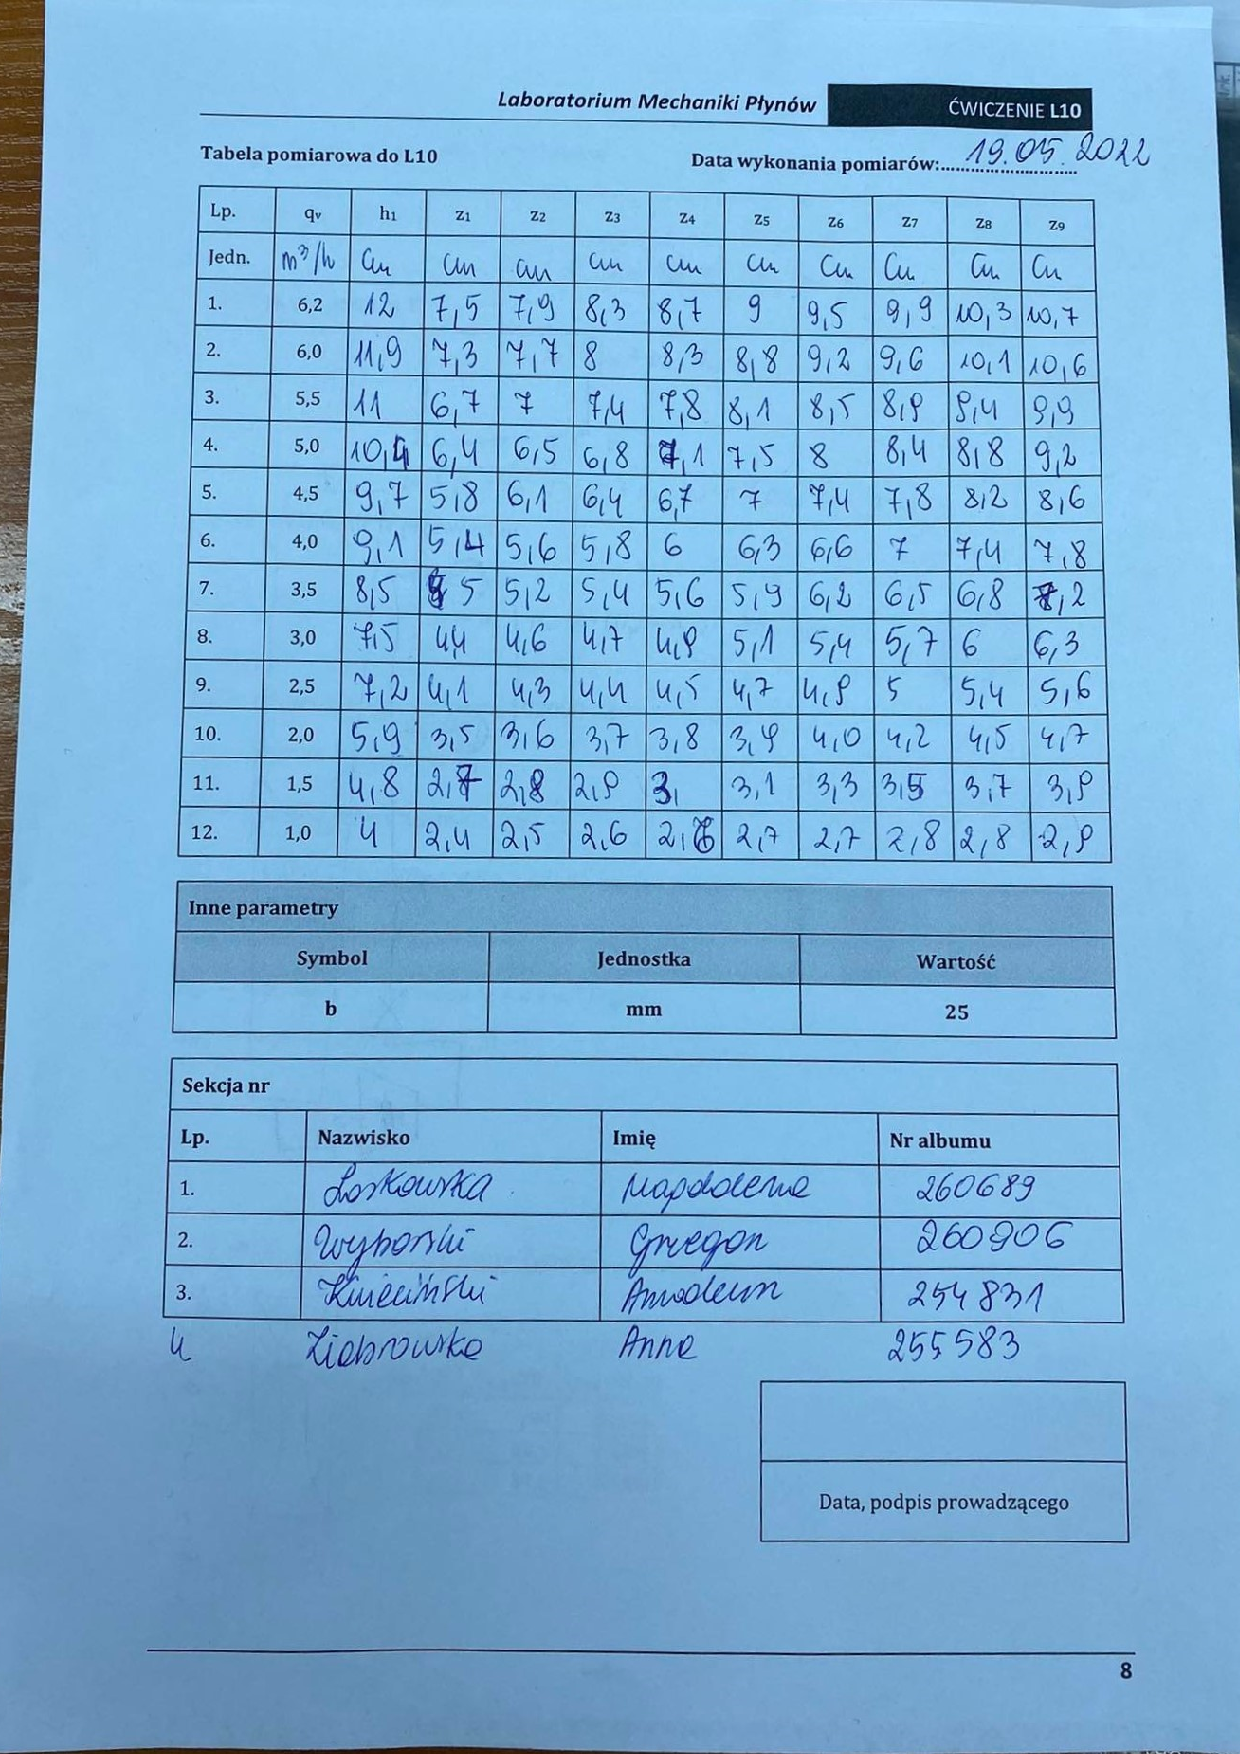
\includepdf{Figures/PDF/Protokol_pomiarowy.pdf}

    \tableofcontents
    % \listoffigures
    % \listoftables
    % \begin{landscape}
    %     \begin{figure}
    %         \section{Stanowisko pomiarowe}
    %         \centering
    %         \includegraphics[width=\linewidth-142px]
    %             {Figures/PDF/Stanowisko_pomiarowe.pdf}
    %             \caption{Shemat budowy stanowiska pomiarowego z wyszczególnionymi elementami oraz pokazanym sposobem podlączenia.}
    %     \end{figure}
    % \end{landscape}

    \pagebreak

    \section{Wstęp}
        \subsection{Opis wymiennika}

\paragraph{}{
    Projektowany będzie wymiennika typu ``Rura w rurze - rury gięte``, jest to modyfikacja wymiennika typu ``Rura w rurze - rury proste``. 
    Stosowany jest w sytuacjach kiedy nie mamy wystarczającej ilości miejsca na zbudowanie klasycznego wymiwnnika z rurami prostymi. Dzięki swoim stosunkowo małym rozmiarą wymiennik ten znalazł zastosowanie w urządzeniach chłodniczych takicha jak lodówki. 
    Przestrzeń wewnątrz wymiennika moża być z łatwoącią zagospodarowana przez umieszczenie wewnątrz zbiornika naczynnik, sprężarki lub innego urządzenia.
    Jego największą wadą jest to, że w trakcie procesu zginania wewętrzna rura może wejś kontakt z rurą zewnętrzną od strony gięcia.
    Taka sytuacja  tworzy przestrzeń w której nie zachodzi wymiana ciepłą między czynnikami.
    Problem ten rozwiązuje się umieszczają pomiędzy rurami różne rodzaje dystansów.
}
        \subsection{Założenia projektu}
\begin{itemize}
    \item Odbieranie ciepła od toluenu w temperaturze 75\(\DEGc\)
    \item Czynnikiem chłodzącym jest woda o temperaturze 10\(\DEGc\)
    \item Przepływ czynnika chłodzącego ma zawierać się w przedziale 0.5 - 1 \(\FLOWRATEkgs\)
    \item Zapobiec stykaniu się ścianek wymiennika
    \item Całkowite wymiary wymiennika mają być jak najmniejsze
    \item Zminimalizować koszta materiału i wykonania
\end{itemize}
        \subsection{Wybór materiałów}    
        \subsection{Rysunki}
\paragraph{}{}

    
    \pagebreak

    \section{Charakterystyka techniczna}
        \subsection{Dane wejsciowe}

    \begin{enumerate}
        \item 
            \begin{flushleft}
                Parametry cieczy schładzanej
                \begin{itemize}
                    \item Toulen
                    \item Temperatura wejściowa \(T_{1we} = 75\DEGc\)
                    \item Temperatura wyjściowa \(T_{1wy} = 55\DEGc\)
                    \item Strumień przepływu    \(Q_{1} = 0.5-1\FLOWRATEs\)
                    \item Dodatkowe parametry czynnika    
                        \begin{figure}[h]
                            \centering
                            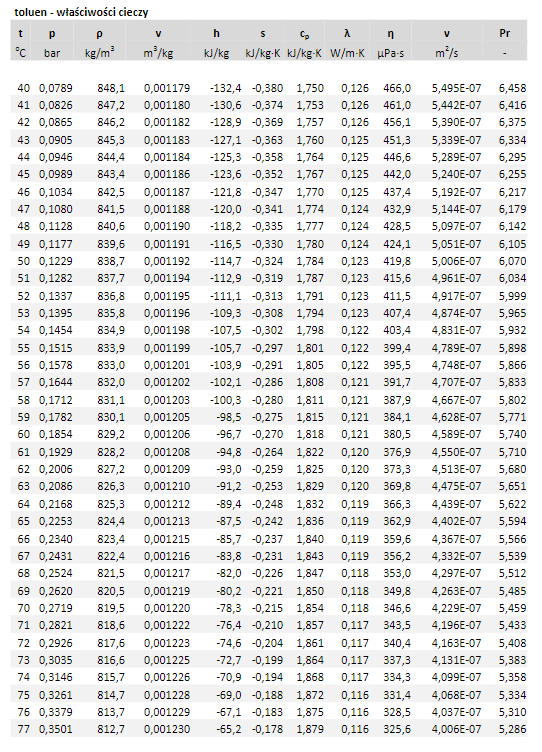
\includegraphics[width=\linewidth-110px]{Tabela_toluen.PNG}
                        \end{figure}
                \end{itemize}
            \end{flushleft} 
        \pagebreak
        \item 
            \begin{flushleft}
                Parametry cieczy chlodzącej
                \begin{itemize}
                    \item Woda
                    \item Temperatura wejściowa \(T_{2we} = 10\DEGc\)
                    \item Temperatura wyjściowa \(T_{2wy} = 30\DEGc\)
                    \item Strumień przepływu    \(Q_{2} = 3\FLOWRATEs\)
                    \item Dodatkowe parametry czynnika
                        \begin{figure}[h]
                            \centering
                            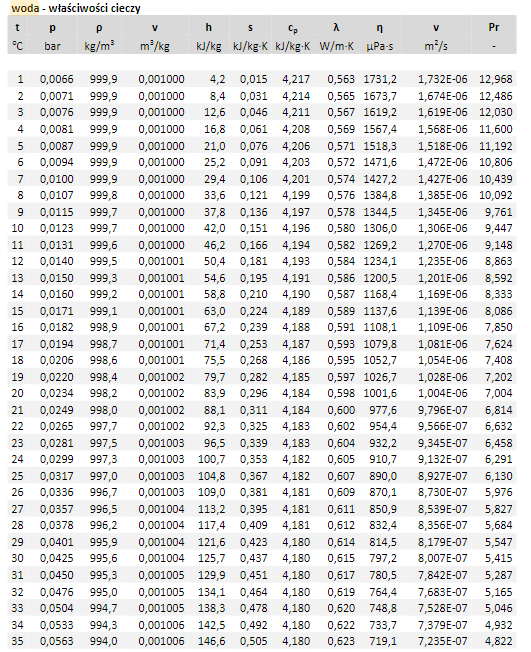
\includegraphics[width=\linewidth-110px]{Tabela_woda.PNG}
                        \end{figure}
                    \end{itemize}
            \end{flushleft}
        \pagebreak    
    \end{enumerate}
    


        \subsection{Dokładne parametry materiałów}
\begin{itemize}
    \item Główny materiał wymiennika: Aluminium AW-1050 \\
    Własności wytrzymałościowe materiału wg normy DIN EN 755-2\\
    Parametry termodynamiczne materiału wg artykułu\href{https://www.azom.com/article.aspx?ArticleID=2798}{Amuminium 1050}
    
    \item Materiał króćców: Mosiądz CW501L\\
    Własności wytrzymałościowe materiału wg normy DIN EN 12163
\end{itemize}    
        \subsection{Podsumowanie}
        % \subsection{Wykresy przepływu}

     
    %\bibliographystyle{plain} 
    %\bibliography{main}
\end{document}